\documentclass[aspectratio=169,usenames,dvipsnames]{beamer}
\usepackage{preamble}
\usepackage{pdfpages}


\title{Coding for Humanities}
\author{Andreas van Cranenburgh}
\date{Week 7: Tabular data analysis with Pandas}

\begin{document}
\maketitle


\begin{frame}{Last week}
    Exploratory analysis of one variable

    \vspace{1em}
    Visualizations, plots

    \vspace{1em}
    Pandas Series objects
\end{frame}

\begin{frame}{Program for today}
\tableofcontents
\end{frame}



\section{The Pandas DataFrame}
\frame{\tableofcontents[currentsection]}

\begin{frame}[fragile]{Terminology recap}
    \begin{description}
        \item[variable] an object with a name that holds a value
        \item[function] code that can be called with arguments and returns a value;
                e.g., \lstinline|number = int('42')|
        \item[object] a combination of data and code; e.g., \lstinline|lst = [0, 1,  2]|
            or \lstinline|Text(tokens)|
        \item[attribute] a variable belonging to an object; e.g., \lstinline|lst.append|
        \item[method] an attribute which is a function; e.g., \lstinline|lst.append()|
        \item[module] a library of functions; e.g., \lstinline|import pandas as pd|
    \end{description}
\end{frame}

\begin{frame}[fragile]{Keyword arguments}
    \begin{definition}
        A named \structure{keyword} argument \texttt{keyword=value} \\
        may be given after required positional arguments.
    \end{definition}

Example:
\begin{lstlisting}
pd.Series([0, 1, 2], index=['a', 'b', 'c'])
\end{lstlisting}
\pause

    \begin{description}
        \item[Positional arguments:]
            typically required, order matters, \\
            must come before keywords.
        \item[Keyword arguments:]
            typically optional, order does not matter,\\
            must come after positional arguments.
    \end{description}
\end{frame}

\begin{frame}[fragile]{From Series to DataFrames}
A series:
\begin{lstlisting}
pd.Series([0, 1, 2], index=['a', 'b', 'c'])
\end{lstlisting}

\pause
A DataFrame can be created from a dictionary of columns:
\begin{lstlisting}
In: pd.DataFrame({'A': [0, 1, 2], 'B': [2, 3, 4]}, index=['a', 'b', 'c'])
    A   B
a   0   2
b   1   3
c   2   4
\end{lstlisting}

\pause
Or using Series objects with the same index:
\begin{lstlisting}
A = pd.Series([0, 1, 2], index=['a', 'b', 'c'])
B = pd.Series([2, 3, 4], index=['a', 'b', 'c'])
pd.DataFrame({'A': A, 'B': B})
\end{lstlisting}
\end{frame}


\begin{frame}[fragile]{From DataFrames to Series}
Given a DateFrame, column can be extracted as Series:
\begin{lstlisting}
In: df = pd.DataFrame({'A': [0, 1, 2], 'B': [2, 3, 4]},
                      index=['a', 'b', 'c'])
In: df['A']
a    0
b    1
c    2
Name: A, dtype: int64
\end{lstlisting}
\end{frame}



\section{Exploring the Palmer Penguins with Pandas}
\subsection{Inspecting the dataset}
\frame{\tableofcontents[currentsubsection]}

%{
%\setbeamercolor{background canvas}{bg=}
%\includepdf[pages=-]{output.pdf}
%}

\begin{frame}[fragile]{Importing modules}
\begin{lstlisting}
import pandas as pd
import seaborn as sns
sns.set_style('white')  # other options: darkgrid, whitegrid, ticks
\end{lstlisting}

See \url{https://seaborn.pydata.org/tutorial/aesthetics.html}
\end{frame}

\begin{frame}{The Palmer Penguins}\centering
    
\includegraphics[width=.7\textheight]{fig/palmerpenguins}

    Dataset credit: \url{https://github.com/allisonhorst/palmerpenguins}
\end{frame}

\begin{frame}[fragile]{Inspecting the data file}
The data is in a Comma-Separated Value (CSV) file:
\begin{lstlisting}
fname = '../../../data/palmerpenguins/inst/extdata/penguins_raw.csv'
with open(fname, encoding='utf8') as inp:
    print(inp.read()[:1000], '...')
\end{lstlisting}

\vspace{-1em}
\begin{lstlisting}[style=plainscript]
studyName,Sample Number,Species,Region,Island,Stage,Individual ID,Clutch Completion,Date Egg,Culmen Length (mm),Culmen Depth (mm),Flipper Length (mm),Body Mass (g),Sex,Delta 15 N (o/oo),Delta 13 C (o/oo),Comments
PAL0708,1,Adelie Penguin (Pygoscelis adeliae),Anvers,Torgersen,"Adult, 1 Egg Stage",N1A1,Yes,2007-11-11,39.1,18.7,181,3750,MALE,NA,NA,Not enough blood for isotopes.
PAL0708,2,Adelie Penguin (Pygoscelis adeliae),Anvers,Torgersen,"Adult, 1 Egg Stage",N1A2,Yes,2007-11-11,39.5,17.4,186,3800,FEMALE,8.94956,-24.69454,NA
PAL0708,3,Adelie Penguin (Pygoscelis adeliae),Anvers,Torgersen,"Adult, 1 Egg Stage",N2A1,Yes,2007-11-16,40.3,18,195,3250,FEMALE,8.36821,-25.33302,NA
PAL0708,4,Adelie Penguin (Pygoscelis adeliae),Anvers,Torgersen,"Adult, 1 Egg Stage",N2A2,Yes,2007-11-16,NA,NA,NA,NA,NA,NA,NA,Adult not sampled.
PAL0708,5,Adelie Penguin (Pygoscelis adeliae),Anvers,Torgersen,"Adult, 1 Egg Stage",N3A1,Yes,2007-11-16,36.7,19.3,193,3450,FEMALE,8.76651,-25.32426,NA
PAL0708,6,Adelie Penguin (P ...
\end{lstlisting}
\end{frame}

\begin{frame}[fragile]{Reading files with Pandas}
\begin{lstlisting}
df = pd.read_csv(fname)
# df = pd.read_csv('data.tsv', sep='\t')
# df = pd.read_csv('data.csv', sep=';')
# df = pd.read_excel('data.xlsx')
\end{lstlisting}

\vspace{1em}
NB: \lstinline|df| is a DataFrame object.
The rest of these slides use this DataFrame.
\end{frame}

\begin{frame}[fragile]{The index column}
If the dataset has row labels, specify the index column.

\vspace{1em}
To use the first column (0) as index:
\begin{lstlisting}
df = pd.read_csv('example.csv', index_col=0)
\end{lstlisting}

Can also specify the name of a column in the file:

\begin{lstlisting}
df = pd.read_csv('example.csv', index_col='Name')
\end{lstlisting}

\vspace{1em}
(For the penguins data we use the automatically generated integer index)
\end{frame}

\begin{frame}[fragile]{Writing data with Pandas}
\begin{lstlisting}
df.to_csv('foo.csv')
df.to_excel('foo.xlsx')
\end{lstlisting}
\end{frame}

%\begin{frame}[fragile]{Flipping the tables}
%To flip rows and columns:
%\begin{lstlisting}
%>>> df = df.T
%\end{lstlisting}
%(T for transpose)
%\end{frame}


\begin{frame}[fragile]{Inspecting the shape and columns}
\begin{lstlisting}
In: df.shape  # NB: shape is an attribute, not a function
(344, 17)
\end{lstlisting}

Our data has 344 rows, 17 columns

\begin{lstlisting}
In: df.columns
\end{lstlisting}
\vspace{-1em}
\begin{lstlisting}[style=plain]
Index(['studyName', 'Sample Number', 'Species', 'Region', 'Island', 'Stage',
'Individual ID', 'Clutch Completion', 'Date Egg', 'Culmen Length (mm)',
'Culmen Depth (mm)', 'Flipper Length (mm)', 'Body Mass (g)', 'Sex',
'Delta 15 N (o/oo)', 'Delta 13 C (o/oo)', 'Comments'], dtype='object')
\end{lstlisting}
(Index is a Pandas object which is a special kind of list).
\end{frame}

\begin{frame}[fragile]{Looking at the first 5 rows: head()}
\vspace{-0.5em}
\begin{lstlisting}
In: df.head()
\end{lstlisting}

\vspace{-1em}
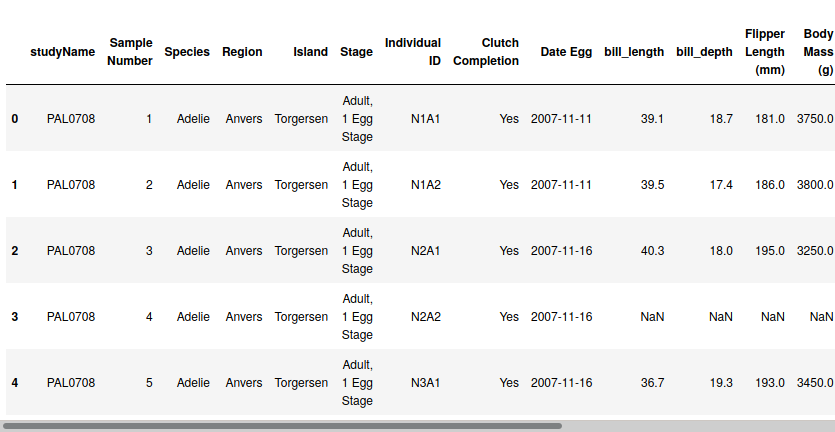
\includegraphics[height=0.8\textheight]{fig/penguinshead}
\end{frame}

\begin{frame}[fragile] %{More information}
\begin{columns}[t]
\column{0.55\textwidth}
    \vspace{-1em}
\begin{lstlisting}[style=script]
In: df.info()
\end{lstlisting}
\vspace{-1em}
\begin{lstlisting}[style=plainscript]
<class 'pandas.core.frame.DataFrame'>
RangeIndex: 344 entries, 0 to 343
Data columns (total 17 columns):
 #   Column               Non-Null Count  Dtype  
---  ------               --------------  -----  
 0   studyName            344 non-null    object 
 1   Sample Number        344 non-null    int64  
 2   Species              344 non-null    object 
 3   Region               344 non-null    object 
 4   Island               344 non-null    object 
 5   Stage                344 non-null    object 
 6   Individual ID        344 non-null    object 
 7   Clutch Completion    344 non-null    object 
 8   Date Egg             344 non-null    object 
 9   Culmen Length (mm)   342 non-null    float64
 10  Culmen Depth (mm)    342 non-null    float64
 11  Flipper Length (mm)  342 non-null    float64
 12  Body Mass (g)        342 non-null    float64
 13  Sex                  333 non-null    object 
 14  Delta 15 N (o/oo)    330 non-null    float64
 15  Delta 13 C (o/oo)    331 non-null    float64
 16  Comments             54 non-null     object 
dtypes: float64(6), int64(1), object(10)
memory usage: 45.8+ KB
\end{lstlisting}
\column{0.45\textwidth}
    \begin{itemize}
        \item Not many missing values (good)
        \item Datatypes (Dtype):
        \begin{itemize}\item boolean, \item integer, \item floating point, \item and object (strings)\end{itemize}
    \end{itemize}
\end{columns}
\end{frame}

\begin{frame}[fragile]{Summary statistics}
\begin{lstlisting}
In: df.describe()
\end{lstlisting}

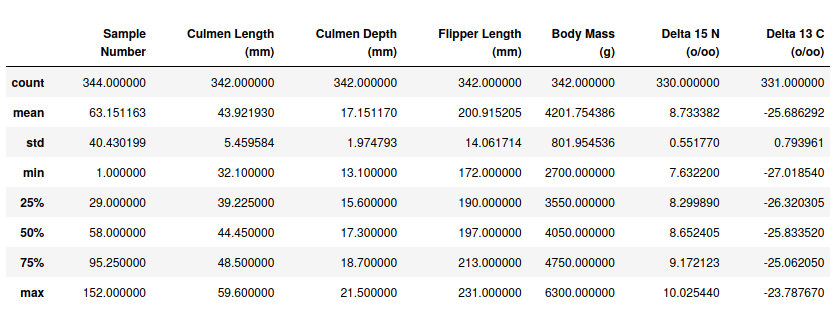
\includegraphics[height=0.7\textheight]{fig/penguinsdescribe}
\end{frame}

\begin{frame}[fragile]{Selecting a column}
\begin{lstlisting}
In: df['Species']
\end{lstlisting}
\vspace{-1em}
\begin{lstlisting}[style=plain]
0            Adelie Penguin (Pygoscelis adeliae)
1            Adelie Penguin (Pygoscelis adeliae)
2            Adelie Penguin (Pygoscelis adeliae)
3            Adelie Penguin (Pygoscelis adeliae)
4            Adelie Penguin (Pygoscelis adeliae)
                         ...                    
339    Chinstrap penguin (Pygoscelis antarctica)
340    Chinstrap penguin (Pygoscelis antarctica)
341    Chinstrap penguin (Pygoscelis antarctica)
342    Chinstrap penguin (Pygoscelis antarctica)
343    Chinstrap penguin (Pygoscelis antarctica)
Name: Species, Length: 344, dtype: object
\end{lstlisting}

Selecting a column returns a Series object
\end{frame}


\begin{frame}[fragile]{Meet the penguins}
\begin{reference}
Image credit: \url{https://github.com/allisonhorst/palmerpenguins}
\end{reference}
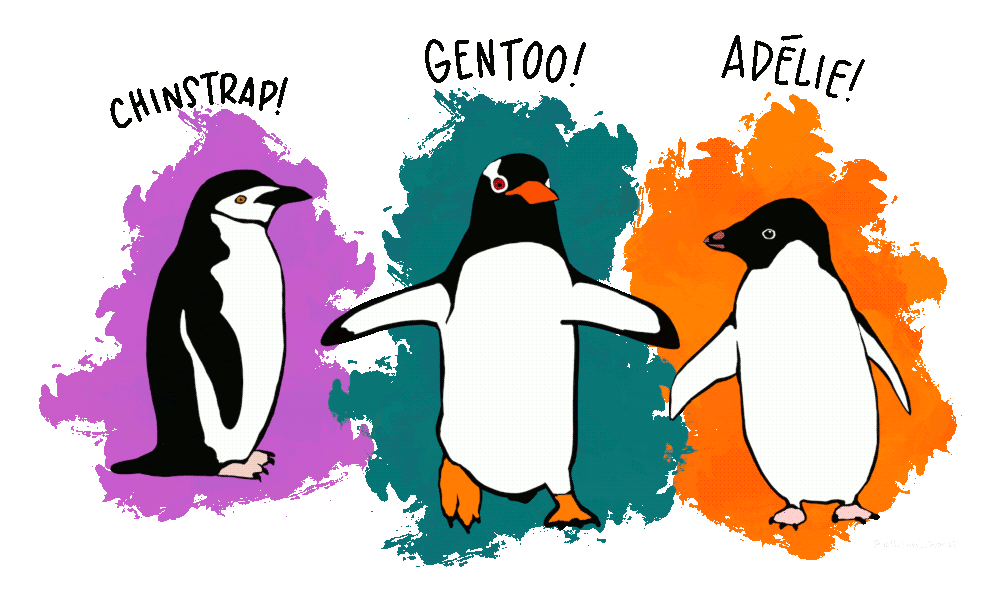
\includegraphics[height=0.4\textheight]{fig/lter_penguins}

Count penguin species:
\begin{lstlisting}
In: df['Species'].value_counts()
\end{lstlisting}
\vspace{-1em}
\begin{lstlisting}[style=plain]
Adelie Penguin (Pygoscelis adeliae)          152
Gentoo penguin (Pygoscelis papua)            124
Chinstrap penguin (Pygoscelis antarctica)     68
Name: Species, dtype: int64
\end{lstlisting}

\end{frame}

\begin{frame}[fragile]{Proportions instead of counts}
\begin{lstlisting}
In: df['Species'].value_counts(normalize=True)
\end{lstlisting}\vspace{-1em}\begin{lstlisting}[style=plain]
Adelie Penguin (Pygoscelis adeliae)          0.441860
Gentoo penguin (Pygoscelis papua)            0.360465
Chinstrap penguin (Pygoscelis antarctica)    0.197674
Name: Species, dtype: float64
\end{lstlisting}
\end{frame}


\subsection{Manipulating and summarizing the data}
\frame{\tableofcontents[currentsubsection]}
\begin{frame}[fragile]{Sorting by a column}
\begin{lstlisting}
In: df.sort_values(by='Body Mass (g)', ascending=False).head()
\end{lstlisting}

\vspace{-1em}
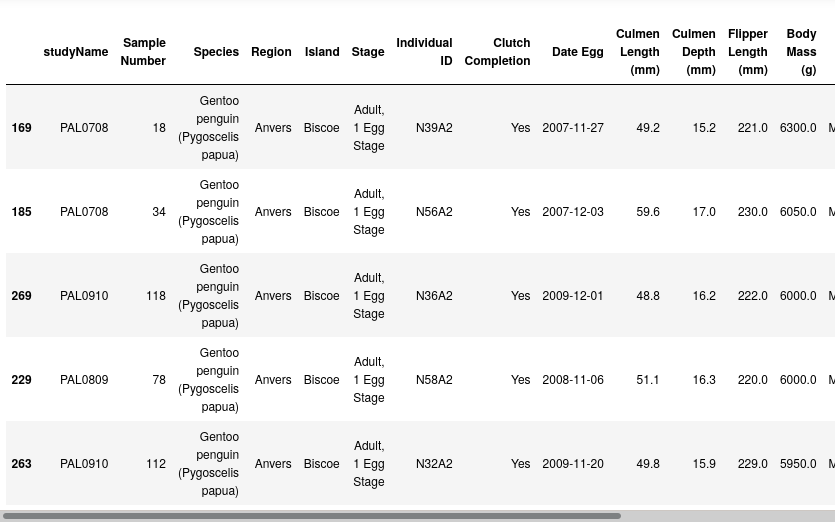
\includegraphics[height=0.7\textheight]{fig/penguinsort}

\lstinline|ascending=False| to sort from high to low
\end{frame}


\begin{frame}[fragile]{Selecting slices of rows/columns (result is a new DataFrame)}
    \begin{itemize}
        \item Selecting rows, columns by label:
\begin{lstlisting}
In: df.loc[0:5, 'Species':'Stage']
\end{lstlisting}

            NB: last element of slice is included!

        \item Selecting rows, columns by integer location:
\begin{lstlisting}
In: df.iloc[0:5, 2:5]
\end{lstlisting}

\vspace{-1em}
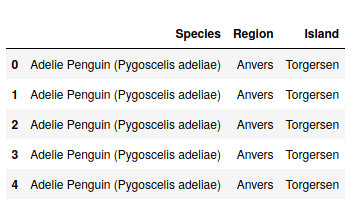
\includegraphics[height=0.4\textheight]{fig/penguinslice}

			NB: last element of slice excluded as usual with Python
    \end{itemize}

\end{frame}

\begin{frame}[fragile]{Boolean operations}
Which rows are male penguins?

\begin{lstlisting}
In: df['Sex'] == 'MALE'
\end{lstlisting}\vspace{-1em}\begin{lstlisting}[style=plain]
0       True
1      False
2      False
3      False
4      False
...  
339     True
340    False
341     True
342     True
343    False
Name: Sex, Length: 344, dtype: bool
\end{lstlisting}
\end{frame}

\begin{frame}[fragile]{Selecting particular rows with a boolean mask}
\vspace{-0.5em}
\begin{lstlisting}
In: df.loc[df['Sex'] == 'MALE', :].head()
\end{lstlisting}

\vspace{-1em}
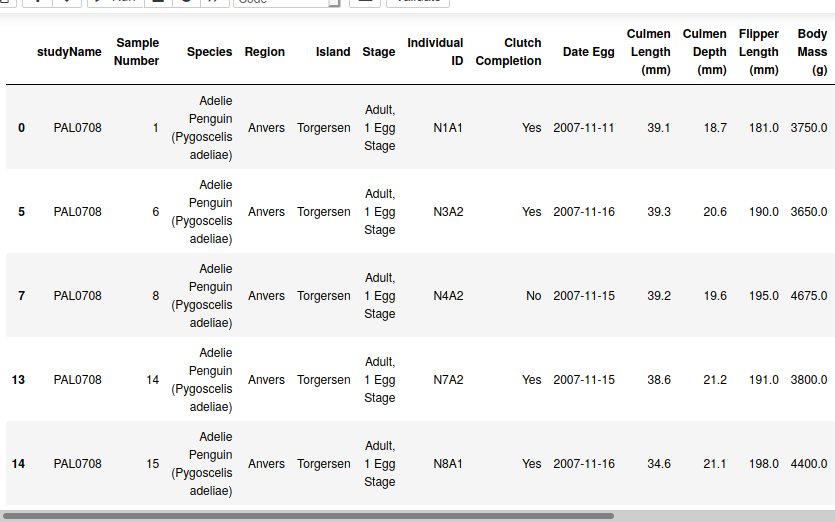
\includegraphics[height=0.8\textheight]{fig/penguinsmale}
\end{frame}

\begin{frame}[fragile]{What are the averages for those penguins?}
\vspace{-0.5em}
\begin{lstlisting}
In: df.loc[df['Sex'] == 'MALE', :].mean()
\end{lstlisting}\vspace{-1em}\begin{lstlisting}[style=plain]
Sample Number            64.148810
Culmen Length (mm)       45.854762
Culmen Depth (mm)        17.891071
Flipper Length (mm)     204.505952
Body Mass (g)          4545.684524
Delta 15 N (o/oo)         8.805398
Delta 13 C (o/oo)       -25.684425
dtype: float64
\end{lstlisting}
\end{frame}

\begin{frame}[fragile]{Answering specific questions}
What is the mean weight for male penguins?
\begin{lstlisting}
In: df.loc[df['Sex'] == 'MALE', 'Body Mass (g)'].mean()
4545.684523809524
\end{lstlisting}

\pause
What is the mean weight of male penguins from Tolgersen island?
More complex selections:
\begin{lstlisting}
In: df.loc[
	(df['Sex'] == 'MALE') & (df['Island'] == 'Torgersen'),
	'Body Mass (g)'].mean()
4034.782608695652
\end{lstlisting}
(note the required parentheses)
\end{frame}



% NB: We avoid lambda / higher-order functions!

% \begin{frame}[fragile]{Applying functions to cells, columns, rows}
% \begin{itemize}
%     \item Apply function to each column:
% 
% \begin{lstlisting}
% >>> df.apply(lambda col: col.max())
% 
% State                        WY
% Account length              243
% Area code                   510
% International plan          Yes
% Voice mail plan             Yes
% [...]
% Churn                         1
% dtype: object
% \end{lstlisting}
% 
% \item Apply function to each row: \\
%     \texttt{df.apply(lambda row: row.max(), axis=1)}
% \end{frame}
 
\begin{frame}[fragile]{Renaming column / index labels}
\begin{reference}
Image credit: \url{https://github.com/allisonhorst/palmerpenguins}
\end{reference}
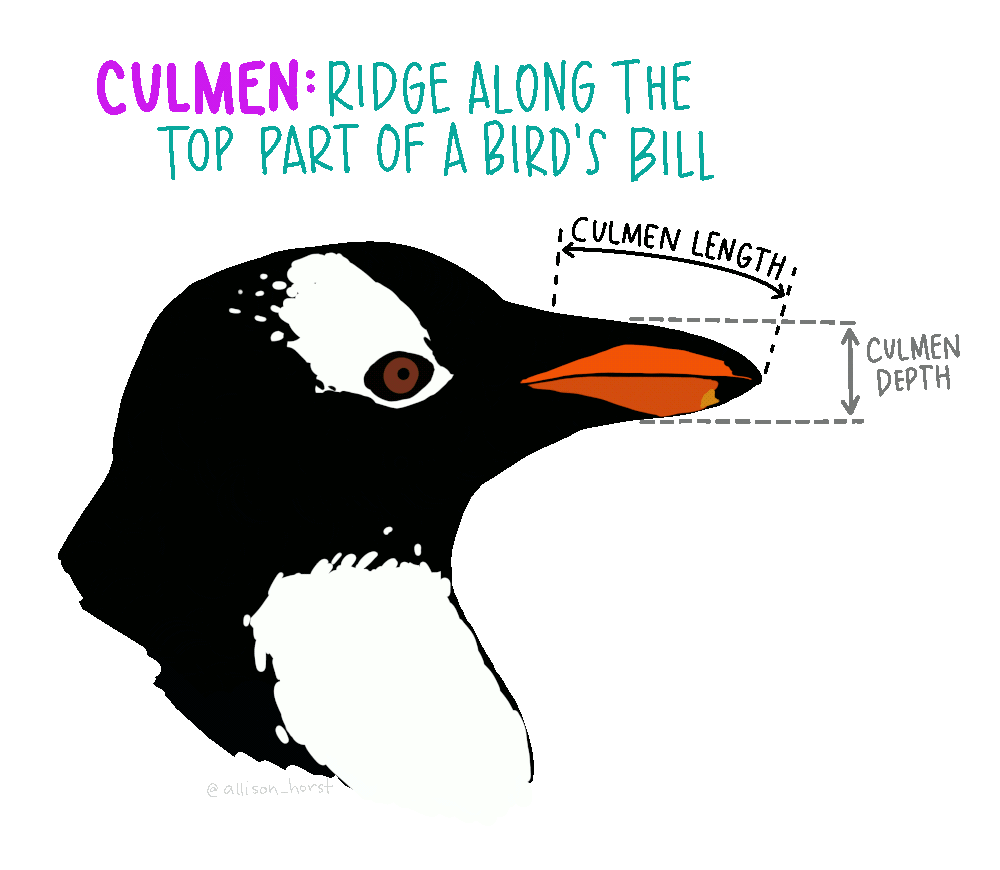
\includegraphics[height=0.5\textheight]{fig/culmen_depth}

Renaming column labels (also works for index):
\begin{lstlisting}
df = df.rename(columns={'Culmen Length (mm)': 'bill_length',
                        'Culmen Depth (mm)': 'bill_depth'})
\end{lstlisting}
\end{frame}

\begin{frame}[fragile]{Replacing values in the table}
Replace values in the \texttt{Species} column with abbreviated species names:
\begin{lstlisting}
# for each (key, value) in repl,
# each occurrence of key is replaced with value
repl = {'Adelie Penguin (Pygoscelis adeliae)': 'Adelie',
        'Gentoo penguin (Pygoscelis papua)': 'Gentoo',
        'Chinstrap penguin (Pygoscelis antarctica)': 'Chinstrap'}
# apply replacements to all values in the 'Species' column
df = df.replace({'Species': repl})
\end{lstlisting}
\end{frame}


\begin{frame}[fragile]{Grouping data (pivot tables)}
Recipe:
\begin{lstlisting}
>>> df.groupby(by=grouping_columns)[columns_to_show].function()
\end{lstlisting}

\begin{enumerate}
\item Create groups based on values in columns specified
    in the list \lstinline{grouping_columns}.
    These will form the rows in the result.
\item Then, select columns of interest (the list \lstinline{columns_to_show}). \\
    If not given, return all other columns.
\item Finally, apply a function to aggregate the data for each group;
    e.g. \lstinline{max(), mean(), describe()}.
\end{enumerate}
\end{frame}


\begin{frame}[fragile]{Grouping example}
\begin{lstlisting}
In: columns_to_show = ['bill_length', 'bill_depth',
                   'Flipper Length (mm)', 'Body Mass (g)']
In: df.groupby(['Sex'])[columns_to_show].mean()
\end{lstlisting}\vspace{-1em}\begin{lstlisting}[style=plain]
        bill_length  bill_depth  Flipper Length (mm)  Body Mass (g)
Sex                                                                
FEMALE    42.096970   16.425455           197.363636    3862.272727
MALE      45.854762   17.891071           204.505952    4545.684524
\end{lstlisting}
\end{frame}

\begin{frame}[fragile]{Adding a new column}
\begin{lstlisting}
# NB: this is just an example! Not a proper application of BMI ...
In: df['BMI'] = df['Body Mass (g)'] / df['Flipper Length (mm)'] ** 2
In: df['BMI']
\end{lstlisting}\vspace{-1em}\begin{lstlisting}[style=plain]
0      0.114465
1      0.109839
2      0.085470
3           NaN
4      0.092620
         ...   
339    0.093351
340    0.083325
341    0.101345
342    0.092971
343    0.096291
Name: BMI, Length: 344, dtype: float64
\end{lstlisting}
\end{frame}

\begin{frame}[fragile]{Delete rows / columns}
\begin{lstlisting}
# get rid of just created column
df = df.drop(['BMI'], axis=1)

# delete the first two rows
df = df.drop([0, 1])
\end{lstlisting}
\end{frame}


\subsection{Exploring and visualizing two or more variables}
\frame{\tableofcontents[currentsubsection]}
\begin{frame}{Exploring two variables}
\begin{description}
    \item[If both categorical:]
            contingency table, bar plot with multiple colors
    \item[One categorical, one continuous:] multiple plots.\\
            For each categorical value, plot histogram / boxplot
    \item[Both continuous:]
         scatter plot, look at correlation
\end{description}

\pause\vspace{1em}
More variables? For handful of variables, can make multiple plots

But interactions get too complicated quickly \dots
\end{frame}


\begin{frame}[fragile]{Contingency table: count across two categorical variables}
\begin{lstlisting}
In: pd.crosstab(df['Sex'], df['Island'])
\end{lstlisting}\vspace{-1em}\begin{lstlisting}[style=plain]
Island  Biscoe  Dream  Torgersen
Sex                             
FEMALE      80     61         24
MALE        83     62         23
\end{lstlisting}

\pause
Get proportions:
\begin{lstlisting}
In: pd.crosstab(df['Sex'], df['Island'], normalize=True)
\end{lstlisting}\vspace{-1em}\begin{lstlisting}[style=plain]
Island    Biscoe     Dream  Torgersen
Sex                                  
FEMALE  0.240240  0.183183   0.072072
MALE    0.249249  0.186186   0.069069
\end{lstlisting}
\end{frame}

\begin{frame}[fragile]{Contingency table with proportions and totals}
\begin{lstlisting}
In: pd.crosstab(df['Sex'], df['Island'], normalize=True, margins=True)
\end{lstlisting}\vspace{-1em}\begin{lstlisting}[style=plain]
Island    Biscoe     Dream  Torgersen       All
Sex                                            
FEMALE  0.240240  0.183183   0.072072  0.495495
MALE    0.249249  0.186186   0.069069  0.504505
All     0.489489  0.369369   0.141141  1.000000
\end{lstlisting}
\end{frame}

\begin{frame}[fragile]{Visualizing two categorical variables: bar plot}
\begin{lstlisting}
ax = pd.crosstab(df['Sex'], df['Island']).plot.barh()
ax.figure.savefig('fig/barplotpenguins.pdf')
\end{lstlisting}

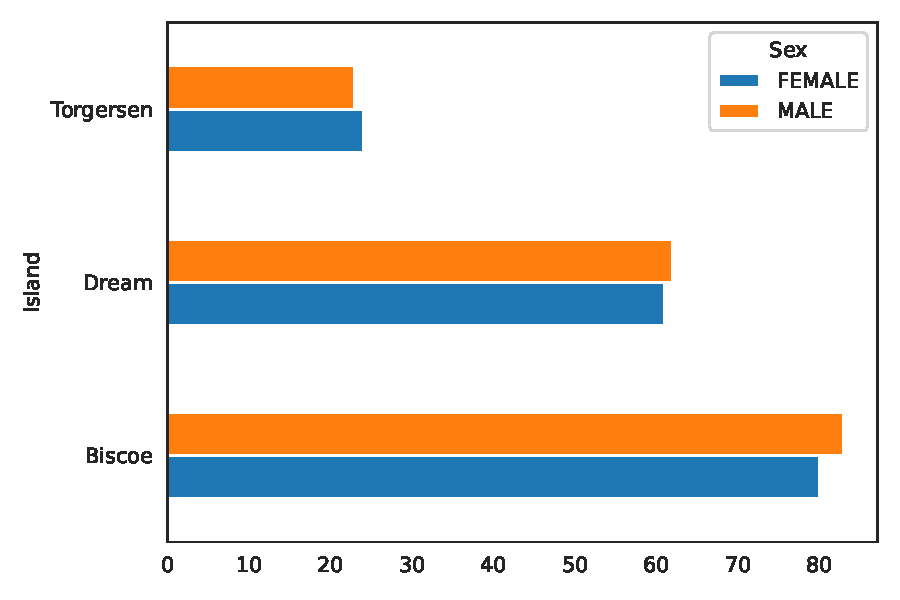
\includegraphics[height=0.7\textheight]{fig/barplotpenguins}
\end{frame}

\begin{frame}[fragile]{One categorical, one continuous variable: box plots}
\begin{lstlisting}
ax = sns.boxplot(x='Body Mass (g)', y='Sex', data=df)
ax.figure.savefig('fig/boxplotpenguins.pdf')
\end{lstlisting}
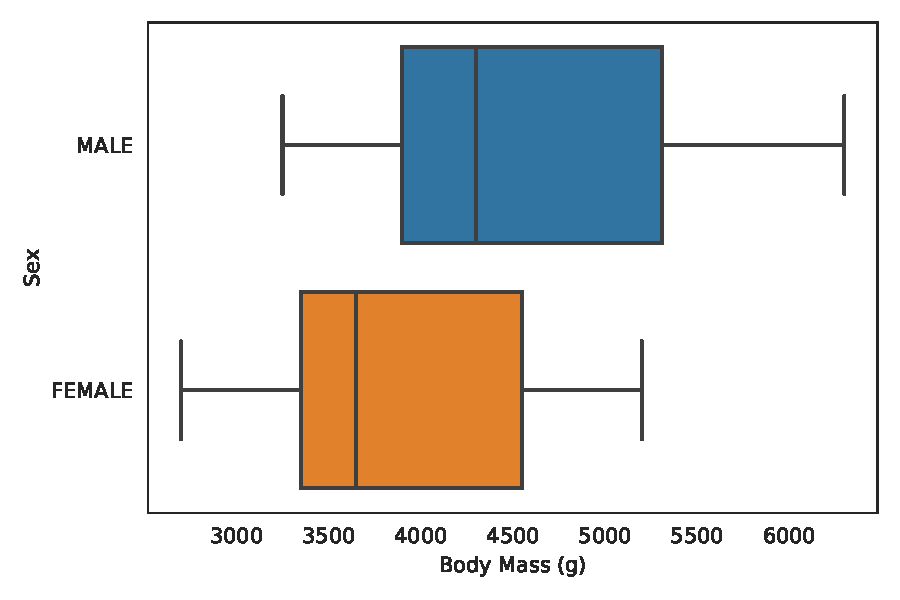
\includegraphics[height=0.7\textheight]{fig/boxplotpenguins}
\end{frame}


\begin{frame}[fragile]{The distribution of a continuous variable: Histogram}
\begin{lstlisting}
fig = sns.displot(x='Flipper Length (mm)', data=df)  # NB: not distplot() !
fig.savefig('fig/histplotpenguins.pdf')
\end{lstlisting}

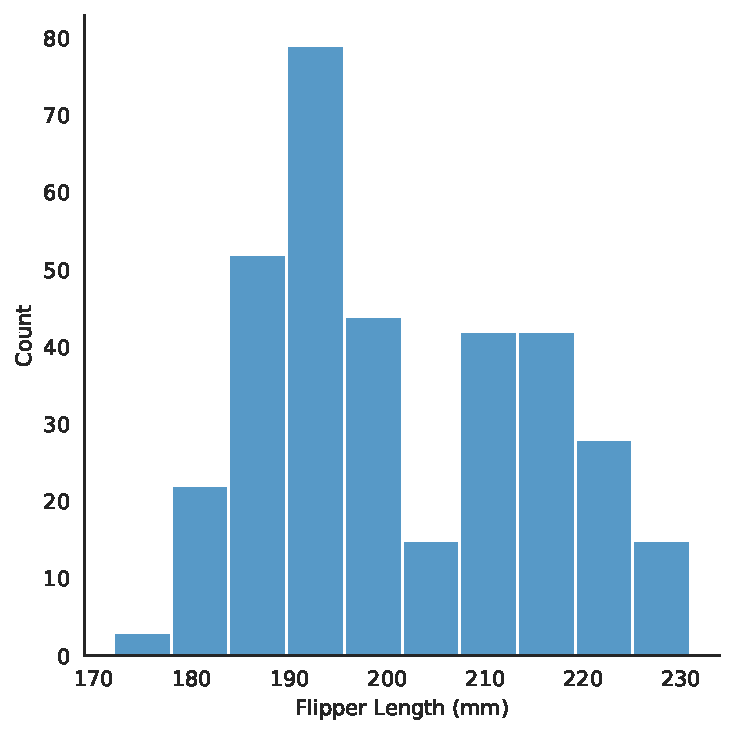
\includegraphics[height=0.7\textheight]{fig/histplotpenguins}
\end{frame}


\begin{frame}[fragile]{One categorical, one continuous variable: Histograms}
\begin{lstlisting}
sns.displot(x='Flipper Length (mm)', col='Species', data=df)
\end{lstlisting}

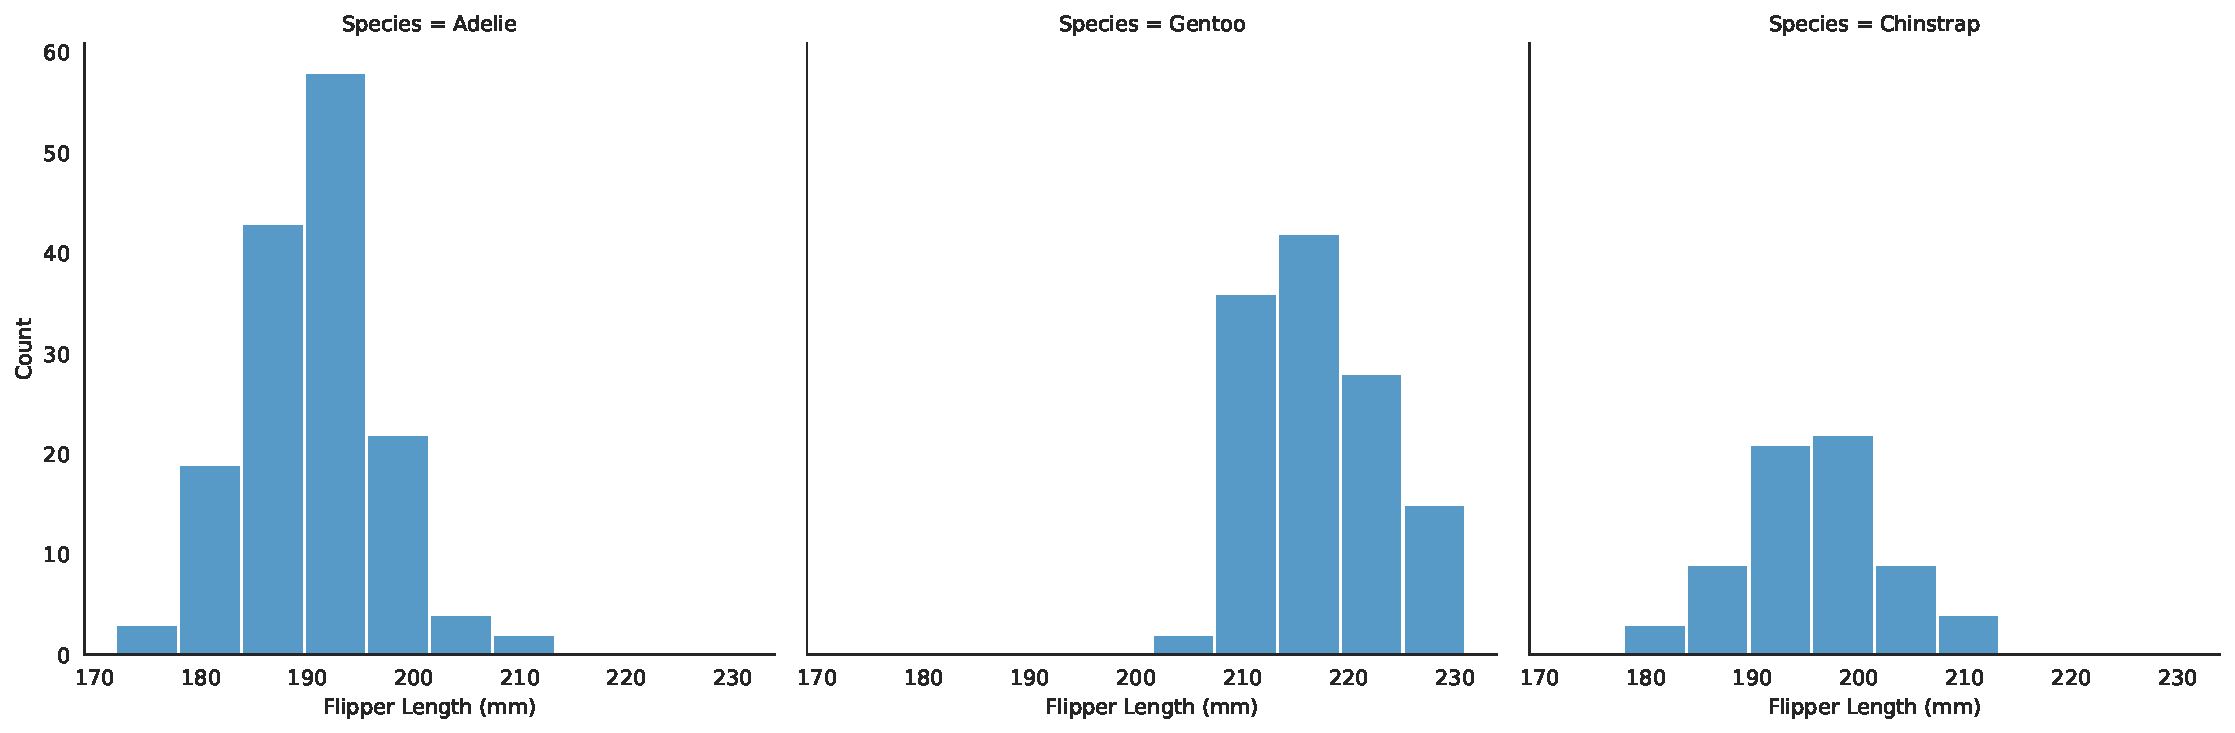
\includegraphics[width=0.9\textwidth]{fig/histplotpenguins1}
\end{frame}


\begin{frame}[fragile]{Two categorical, one continuous variable: Histograms}
\begin{lstlisting}
sns.displot(x='Flipper Length (mm)', col='Species', row='Sex', data=df)
\end{lstlisting}

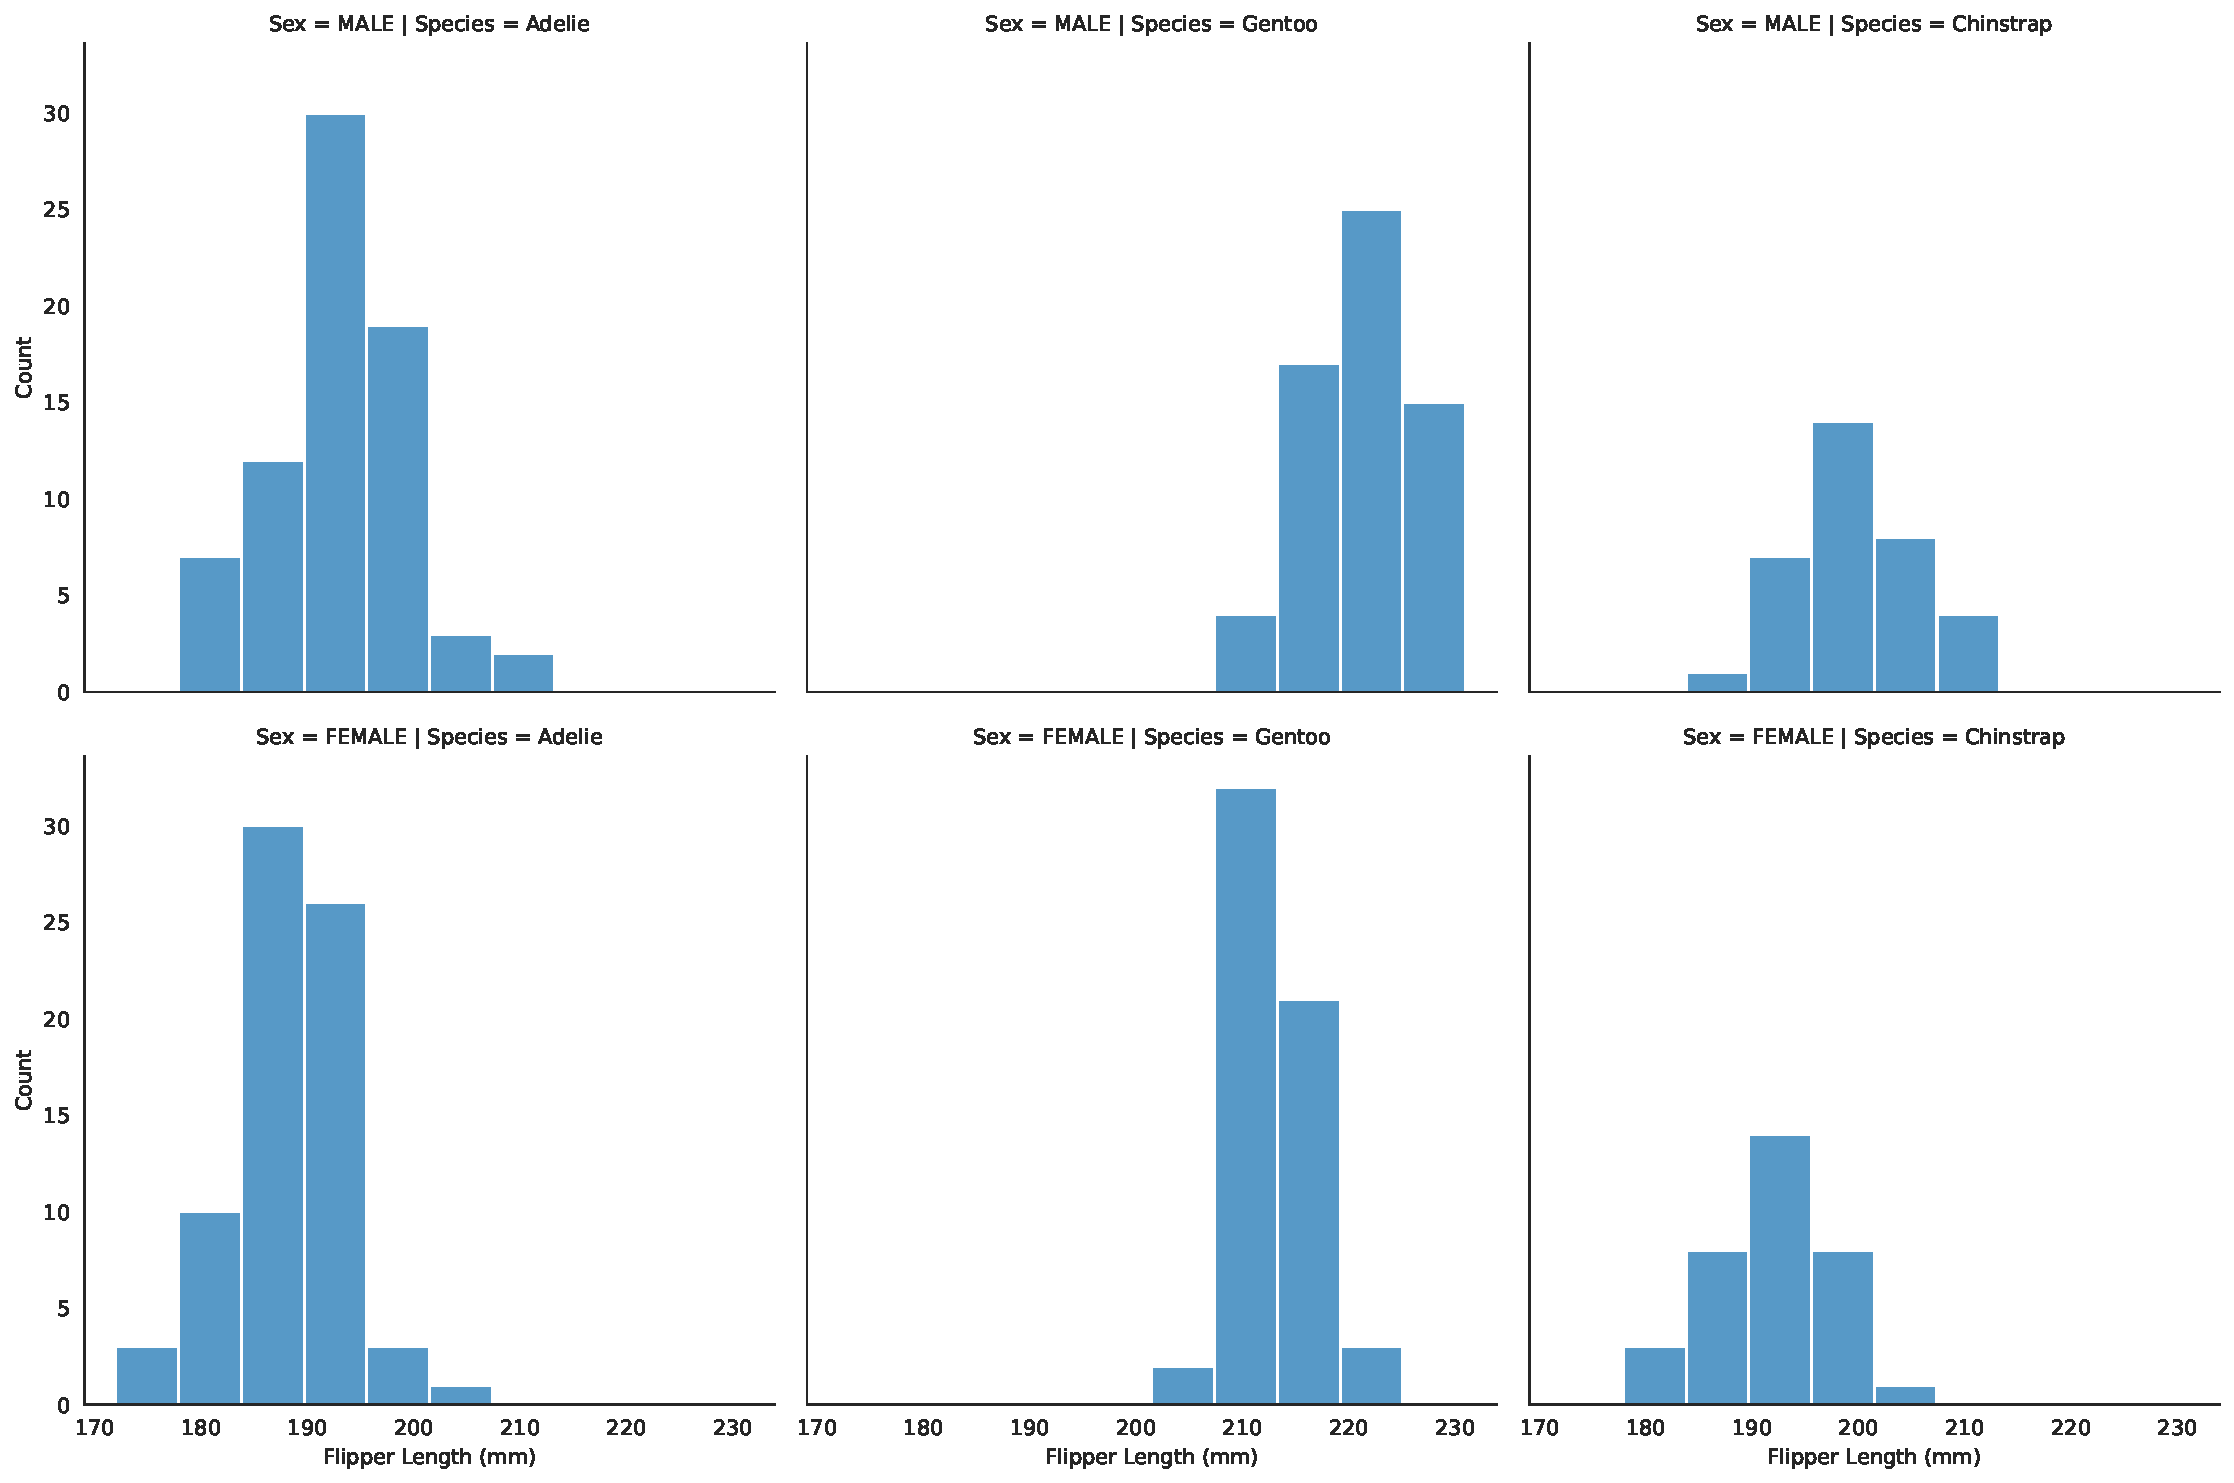
\includegraphics[height=0.75\textheight]{fig/histplotpenguins2}
\end{frame}


\begin{frame}[fragile]{Two continuous variables: scatter plot}
\begin{lstlisting}
sns.relplot(x='Flipper Length (mm)', y='Body Mass (g)', data=df)
\end{lstlisting}

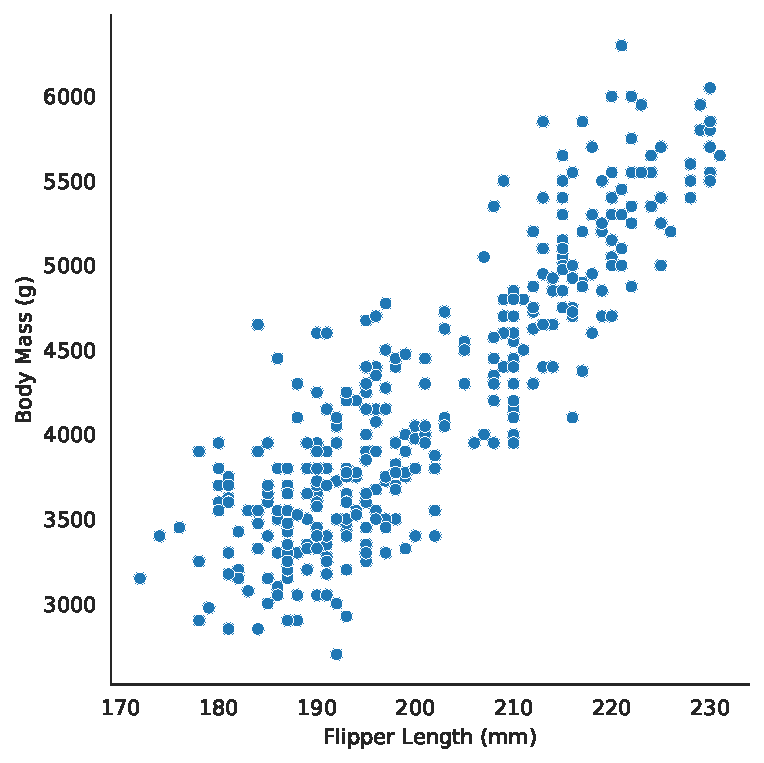
\includegraphics[height=0.7\textheight]{fig/scatterpenguins}
\end{frame}

\begin{frame}[fragile]{Two continuous variables: correlation coefficient}
    \begin{itemize}
        \item Take variables X and Y
        \item If X goes up, does Y tend to go up/down?
        \item How strong is this relationship?
        \item Is the relationship meaningful?
    \end{itemize}

\begin{lstlisting}
In: df['Flipper Length (mm)'].corr(df['Body Mass (g)'])
0.8712017673060114
\end{lstlisting}

\pause\vspace{1em}
Pearson $r$ measures linear association of two variables.

\begin{itemize}
    \item -1 perfect inverse/negative correlation (x goes up, y goes down)
    \item 0 no \structure{linear} relation
    \item 1 perfect positive correlation (x goes up, y goes up)
\end{itemize}

\end{frame}


\begin{frame}[fragile]{Two continuous, one categorical variable: scatter plot}
\vspace{-0.5em}
\begin{lstlisting}
sns.relplot(x='Flipper Length (mm)', y='Body Mass (g)',
            hue='Species', data=df)
\end{lstlisting}

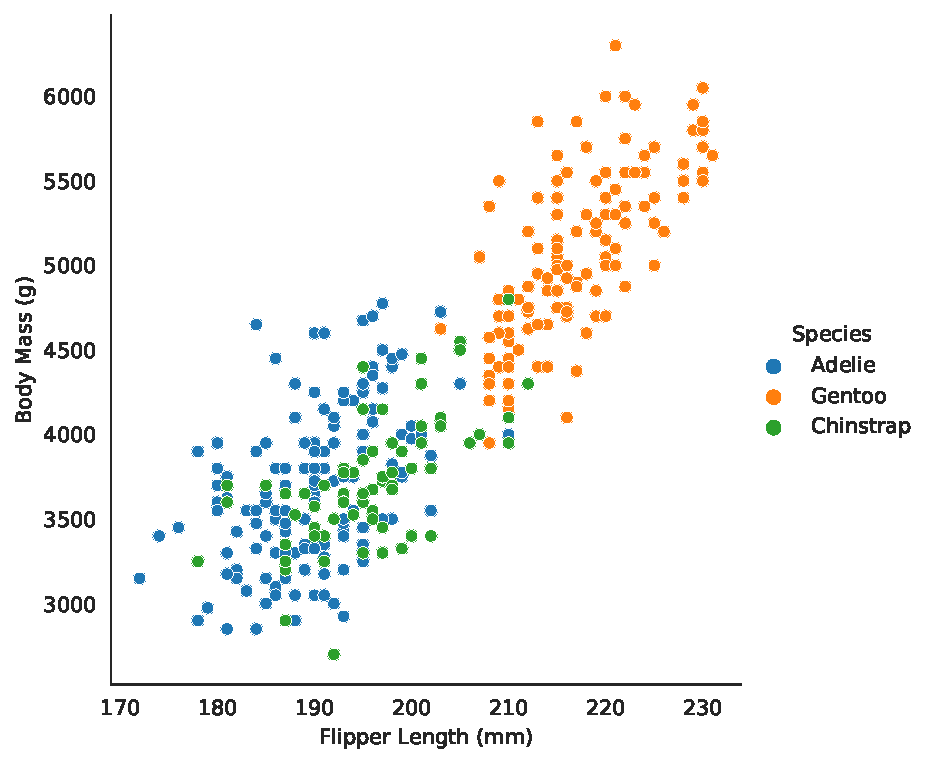
\includegraphics[height=0.7\textheight]{fig/scatterpenguins1}
\end{frame}

\begin{frame}[fragile]{A linear regression plot (with 95\% confidence intervals)}
\vspace{-0.5em}
\begin{lstlisting}
sns.lmplot(x='Flipper Length (mm)', y='bill_length',
           hue='Species', markers=['o', '^', 's'], data=df)
\end{lstlisting}

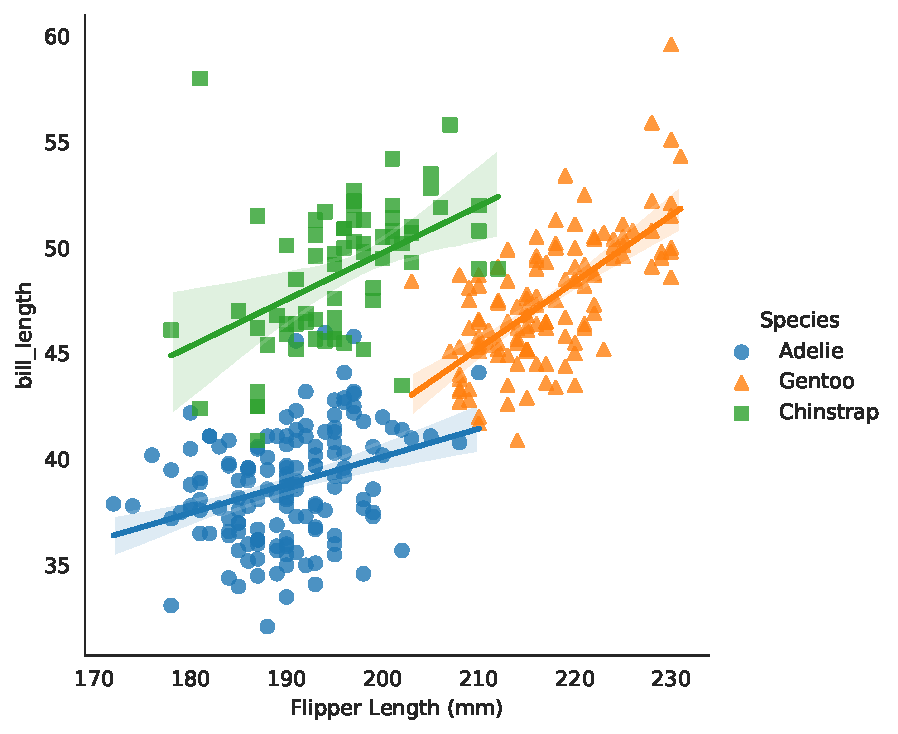
\includegraphics[height=0.7\textheight]{fig/scatterpenguins2}
\end{frame}


%\section{Exploring tabular datasets with Pandas}
%\frame{\tableofcontents[currentsection]}

% From http://swcarpentry.github.io/python-novice-gapminder/
% Reading Tabular Data into DataFrames
%     Use the Pandas library to get basic statistics out of tabular data.
%     Use index_col to specify that a column's values should be used as row headings.
%     Use DataFrame.info to find out more about a dataframe.
%     The DataFrame.columns variable stores information about the dataframe's columns.
%     Use DataFrame.T to transpose a dataframe.
%     Use DataFrame.describe to get summary statistics about data.

% missing: index_col, .T

% Pandas DataFrames
%     Use DataFrame.iloc[..., ...] to select values by integer location.
%     Use : on its own to mean all columns or all rows.
%     Select multiple columns or rows using DataFrame.loc and a named slice.
%     Result of slicing can be used in further operations.
%     Use comparisons to select data based on value.
%     Select values or NaN using a Boolean mask.


% Plotting
%     matplotlib is the most widely used scientific plotting library in Python.
%     Plot data directly from a Pandas dataframe.
%     Select and transform data, then plot it.
%     Many styles of plot are available: see the Python Graph Gallery for more options.
%     Can plot many sets of data together.



%\begin{frame}{Creating a DataFrame}
%\end{frame}

%\begin{frame}{Loading a dataset}
%use pandas.read\_csv()
%%     Use index_col to specify that a column's values should be used as row headings.
% \end{frame}
%\begin{frame}{Basic information}
%     Use DataFrame.info to find out more about a dataframe.
%     The DataFrame.columns variable stores information about the dataframe's columns.
%\end{frame}

%     Use DataFrame.T to transpose a dataframe.
%     Use DataFrame.describe to get summary statistics about data.






















\section{Course overview}
\frame{\tableofcontents[currentsubsection]}

\begin{frame}{The final exam}
    \begin{itemize}
        \item Study all the slides, notebooks, and exercises of week 1--7
        \item Released Thursday 29 Oct 2020, 9:00 morning
        \item Due date Friday 30 Oct 2020, 18:00 evening
    \end{itemize}
\end{frame}

\begin{frame}{Learning goals}
    \begin{enumerate}
        \item Write simple programs to perform basic tasks such as searching
            and cleaning text corpora
        \item Work with Jupyter Notebooks and other common Python data science
            tools to report on simple exploratory experiments:
            load a tabular dataset, compute summary statistics,
            and create plots
        \item Understand and solve common errors during programming
        \item Read documentation on available software to evaluate its
            applicability to a problem
        \item Collaborate effectively with programmers using proper terminology
    \end{enumerate}
\end{frame}

\subsection{Where to go from here}
\frame{\tableofcontents[currentsection]}

\begin{frame}{``Normal'' programming without Notebooks}
    \begin{reference}
        \url{http://www.sublimetext.com/}
        \url{https://notepad-plus-plus.org/}
        \url{https://www.vim.org/}
    \end{reference}
    \begin{columns}[T]
        \column{0.5\linewidth}
            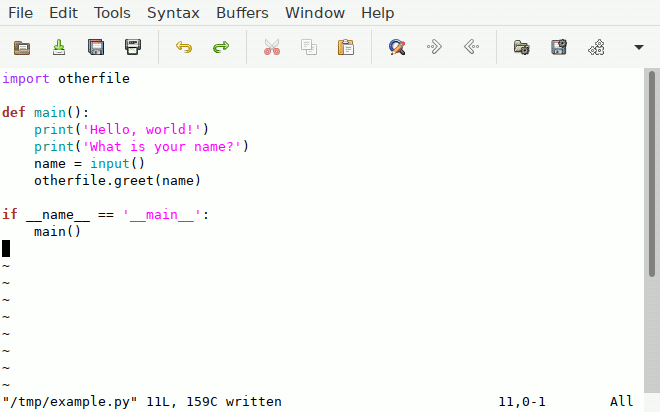
\includegraphics[width=0.9\textwidth]{fig/editor}
            \begin{itemize}
                \item Write code in editor (e.g., Sublime Text, Notepad++, Vim)
                \item Save as plain text in .py files
                \item import functions \\
                    from other .py files
            \end{itemize}
        \pause
        \column{0.5\linewidth}
            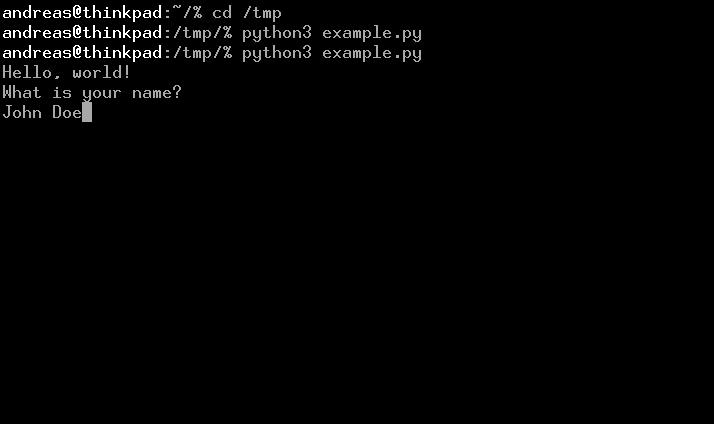
\includegraphics[width=0.9\textwidth]{fig/terminal}
            \begin{itemize}
                \item Run code in a terminal\\
                    (``command prompt'')
            \end{itemize}
    \end{columns}
\end{frame}

\begin{frame}{Jupyter Notebook}
    \begin{block}{Jupyter Notebook}
        A notebook keeps narrative, code, and results together.

        Ideally, everything can be reproduced with the push of a button.
    \end{block}
    \begin{itemize}
        \item Web-based graphical interface
        \item Mix code, results, and explanation \\
                (Knuth: Literate Programming)
        \item Include plots / pictures
        \item Interactive, rapid prototyping
    \end{itemize}

    \pause
    Pros and cons:
    \begin{itemize}
        \item Why Jupyter is data scientists' computational notebook of choice,
            Nature (2018). \url{https://www.nature.com/articles/d41586-018-07196-1}
        \item Why I don't like notebooks, Joel Grus (2018).
            \url{https://www.youtube.com/watch?v=7jiPeIFXb6U}
    \end{itemize}
\end{frame}

\begin{frame}{Notebook pitfalls}
    \begin{columns}
        \column{0.5\linewidth}
            \begin{itemize}
                \item Hidden state and out-of-order execution:\\
                    Ensure code works by running all cells from start to finish!
                    (Kernel $\rightarrow$ Restart \& Run All)
            \end{itemize}
        \column{0.5\linewidth}
            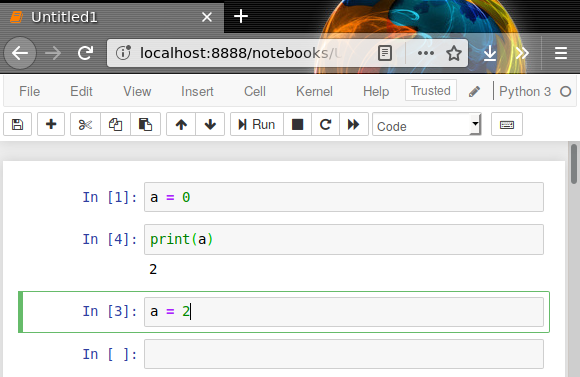
\includegraphics[width=0.95\textwidth]{fig/nboutoforder}
    \end{columns}
    \pause
    \begin{itemize}
        \item Jupyter ``encourages'' throw-away code:\\
                Put re-usable code in a normal Python module and import.
                Apply software engineering practices:
                \begin{itemize}
                    \item Ensure modular, documented code
                    \item Check correctness with tests
                \end{itemize}
        % \pause
        % \item Notebooks can be put into version control, \\
        %         but the differences are hard to read
    \end{itemize}

    Despite this, notebooks are an excellent tool \\
    for exploration and sharing results
\end{frame}



\begin{frame}{Learn more}
    Recommended further materials:
    \vspace{1em}
    \begin{itemize}
        \item \url{https://jakevdp.github.io/PythonDataScienceHandbook/}
        \item \url{https://ProgrammingHistorian.org/en/lessons/}
        \item \url{https://AutomateTheBoringStuff.com/}
    \end{itemize}
\end{frame}


\begin{frame}\Huge\centering
    That's all, folks!
\end{frame}


\begin{frame}
Inspiration for these slides:
\begin{itemize}
\item \url{https://www.cs.umd.edu/class/fall2018/cmsc320/}
    specifically lecture 11
    % https://www.cs.umd.edu/class/fall2018/cmsc320/lecs/cmsc320_f2018_lec11.pdf
\item \url{https://mlcourse.ai/}
    specifically lecture 1
\item \url{https://github.com/allisonhorst/palmerpenguins}
\end{itemize}

\vspace{1em}
Documentation:
\begin{itemize}
    \item \url{https://pandas.pydata.org/pandas-docs/stable/}
    \item \url{https://pandas.pydata.org/pandas-docs/stable/getting_started/comparison/comparison_with_sql.html}
    \item \url{https://seaborn.pydata.org/tutorial.html}
\end{itemize}
\end{frame}

\end{document}









\begin{frame}{House prices \& per capita income}
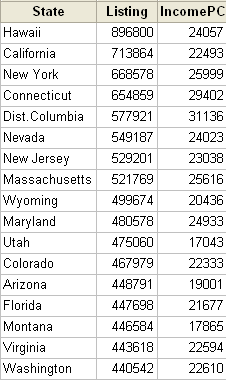
\includegraphics[height=0.85\textheight]{fig/housepricesincome}
\end{frame}

\begin{frame}{Scatter plot suggests positive correlation}
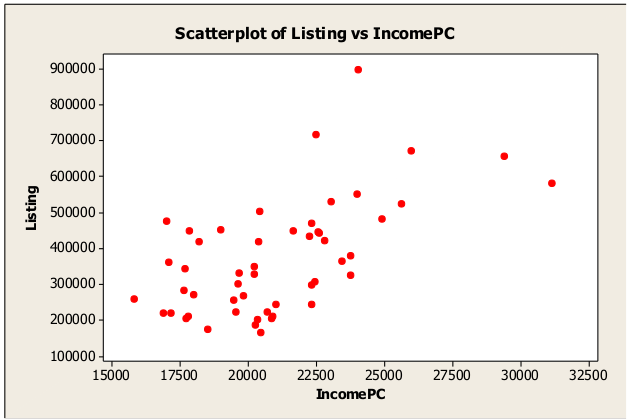
\includegraphics[height=0.7\textheight]{fig/incomelistingscatter}
\end{frame}

\begin{frame}{Correlation is not causation}
Does a rise in income \structure{cause} a rise in gas prices?!

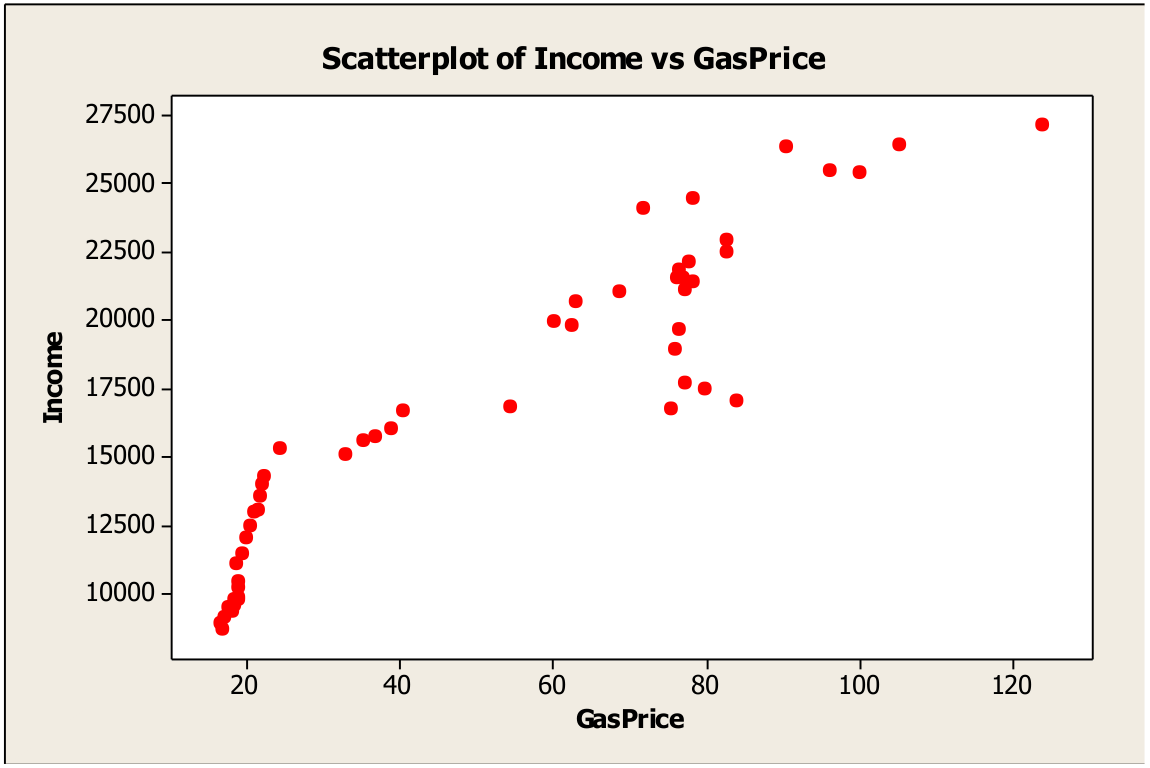
\includegraphics[height=0.7\textheight]{fig/incomegas}

US gasoline prices, 1953-2004, plotted against per-capita US income
\end{frame}

\begin{frame}{Omitted variable: time}
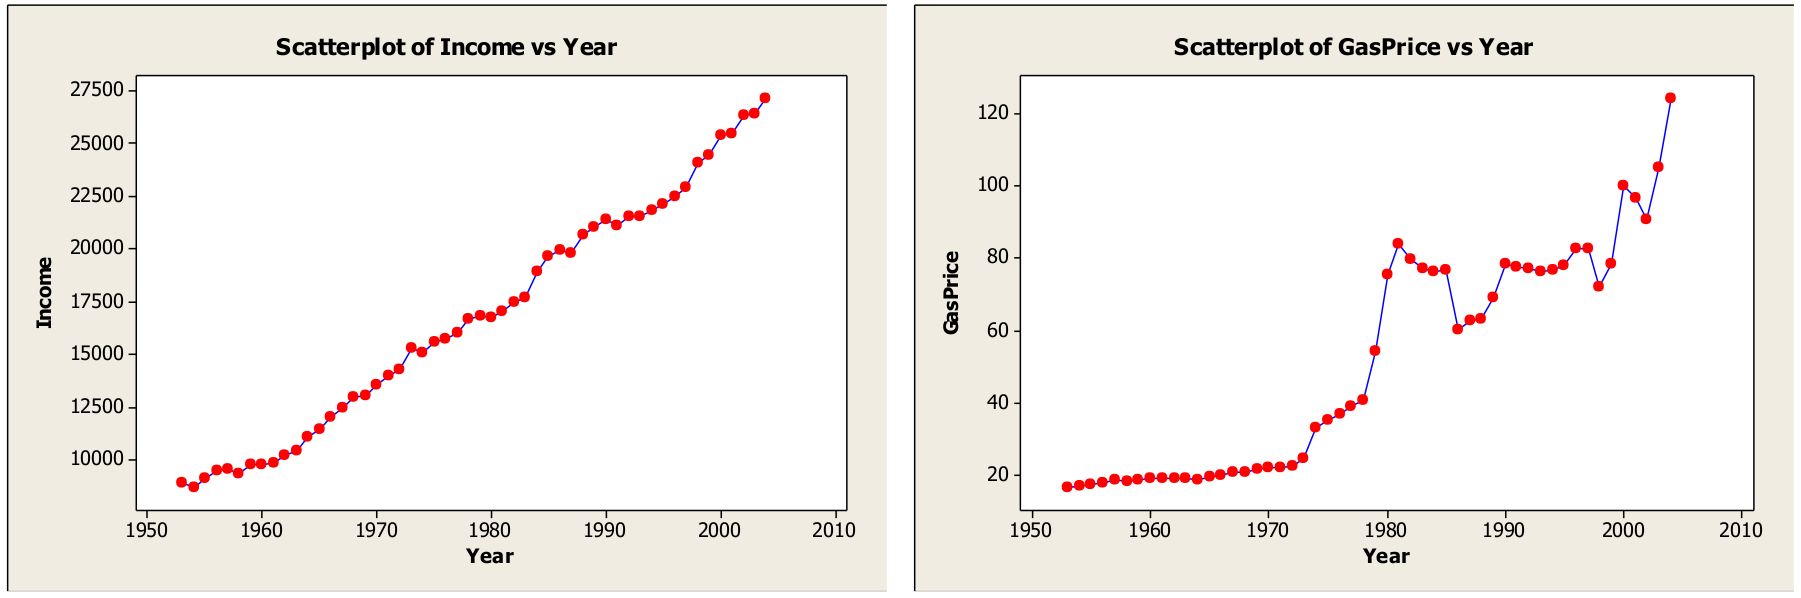
\includegraphics[width=0.99\textwidth]{fig/incomegastime}

No, both income and gas price rise with time (confounding factor).
\end{frame}


\begin{frame}{Pearson's correlation coefficient $r$}
Want to capture:
some variable X varies in the same direction
and at the same scale as some other variable Y

\vspace{1em}
Pearson $r$ measures linear association of two variables.

$r$ is \structure{unitless} in [-1, +1]:

\begin{itemize}
    \item -1 perfect inverse/negative correlation
    \item 0 no \structure{linear} relation
    \item 1 perfect positive correlation
\end{itemize}
\end{frame}

\begin{frame}{House price and income}
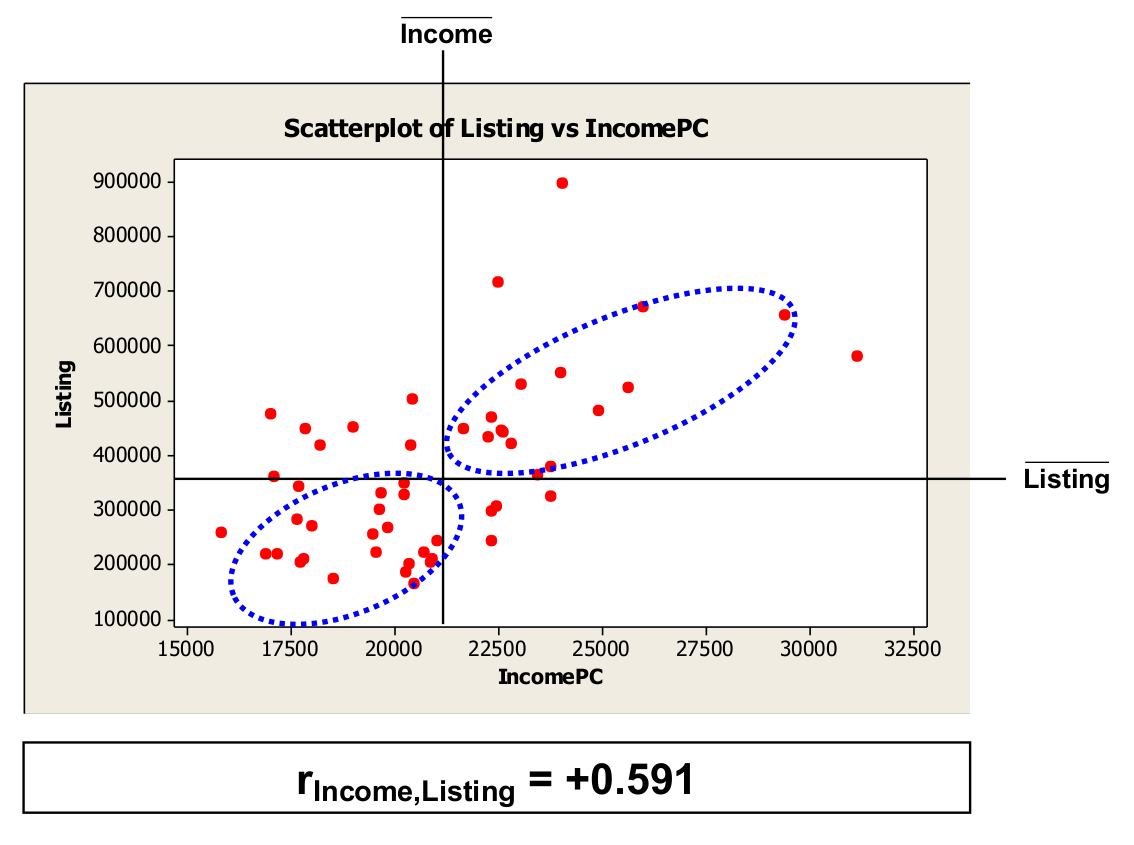
\includegraphics[height=0.8\textheight]{fig/incomelistingcorr}
\end{frame}

\begin{frame}{Examples of $r$}
\begin{reference}\vspace{1em}
Figure: \url{https://en.wikipedia.org/wiki/Correlation_and_dependence}
\end{reference}
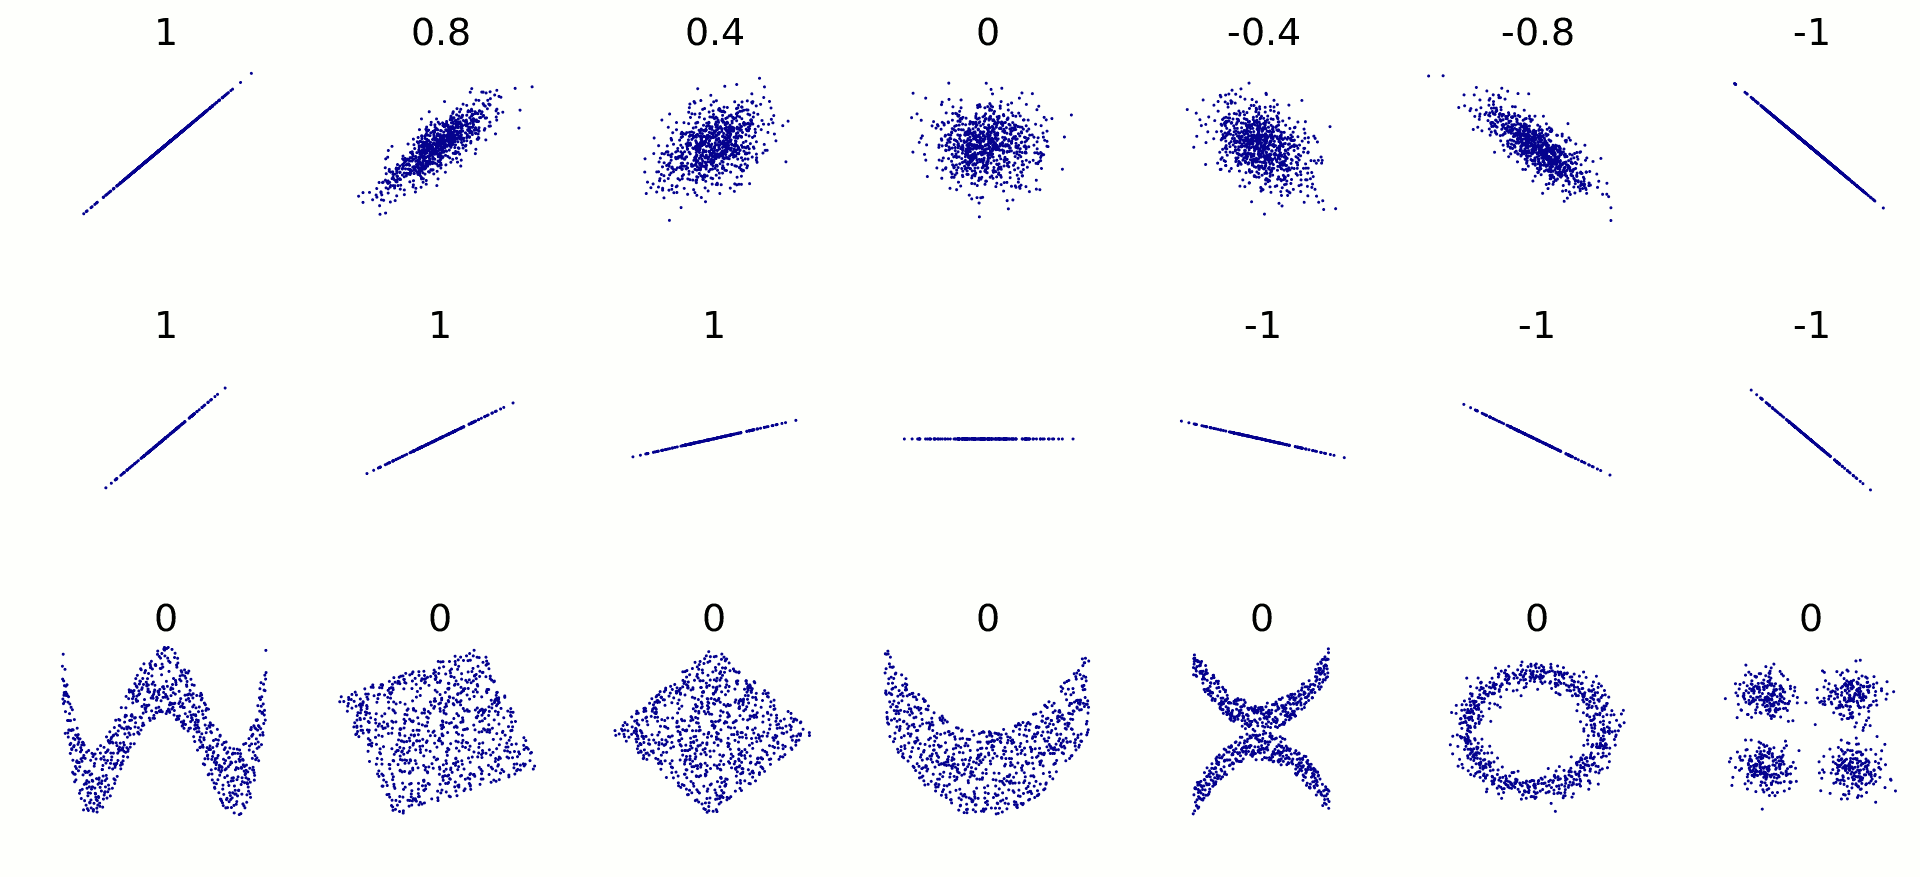
\includegraphics[height=0.6\textheight]{fig/wpcorrelation}

\begin{itemize}
    \item Amount of noise determines strength of correlation
    \item Not slope!
    \item Only linear relationship is measured
\end{itemize}
\end{frame}

\begin{frame}{Correlation is not causation}
\begin{reference}\vspace{1em}
    \url{http://tylervigen.com/spurious-correlations}
\end{reference}
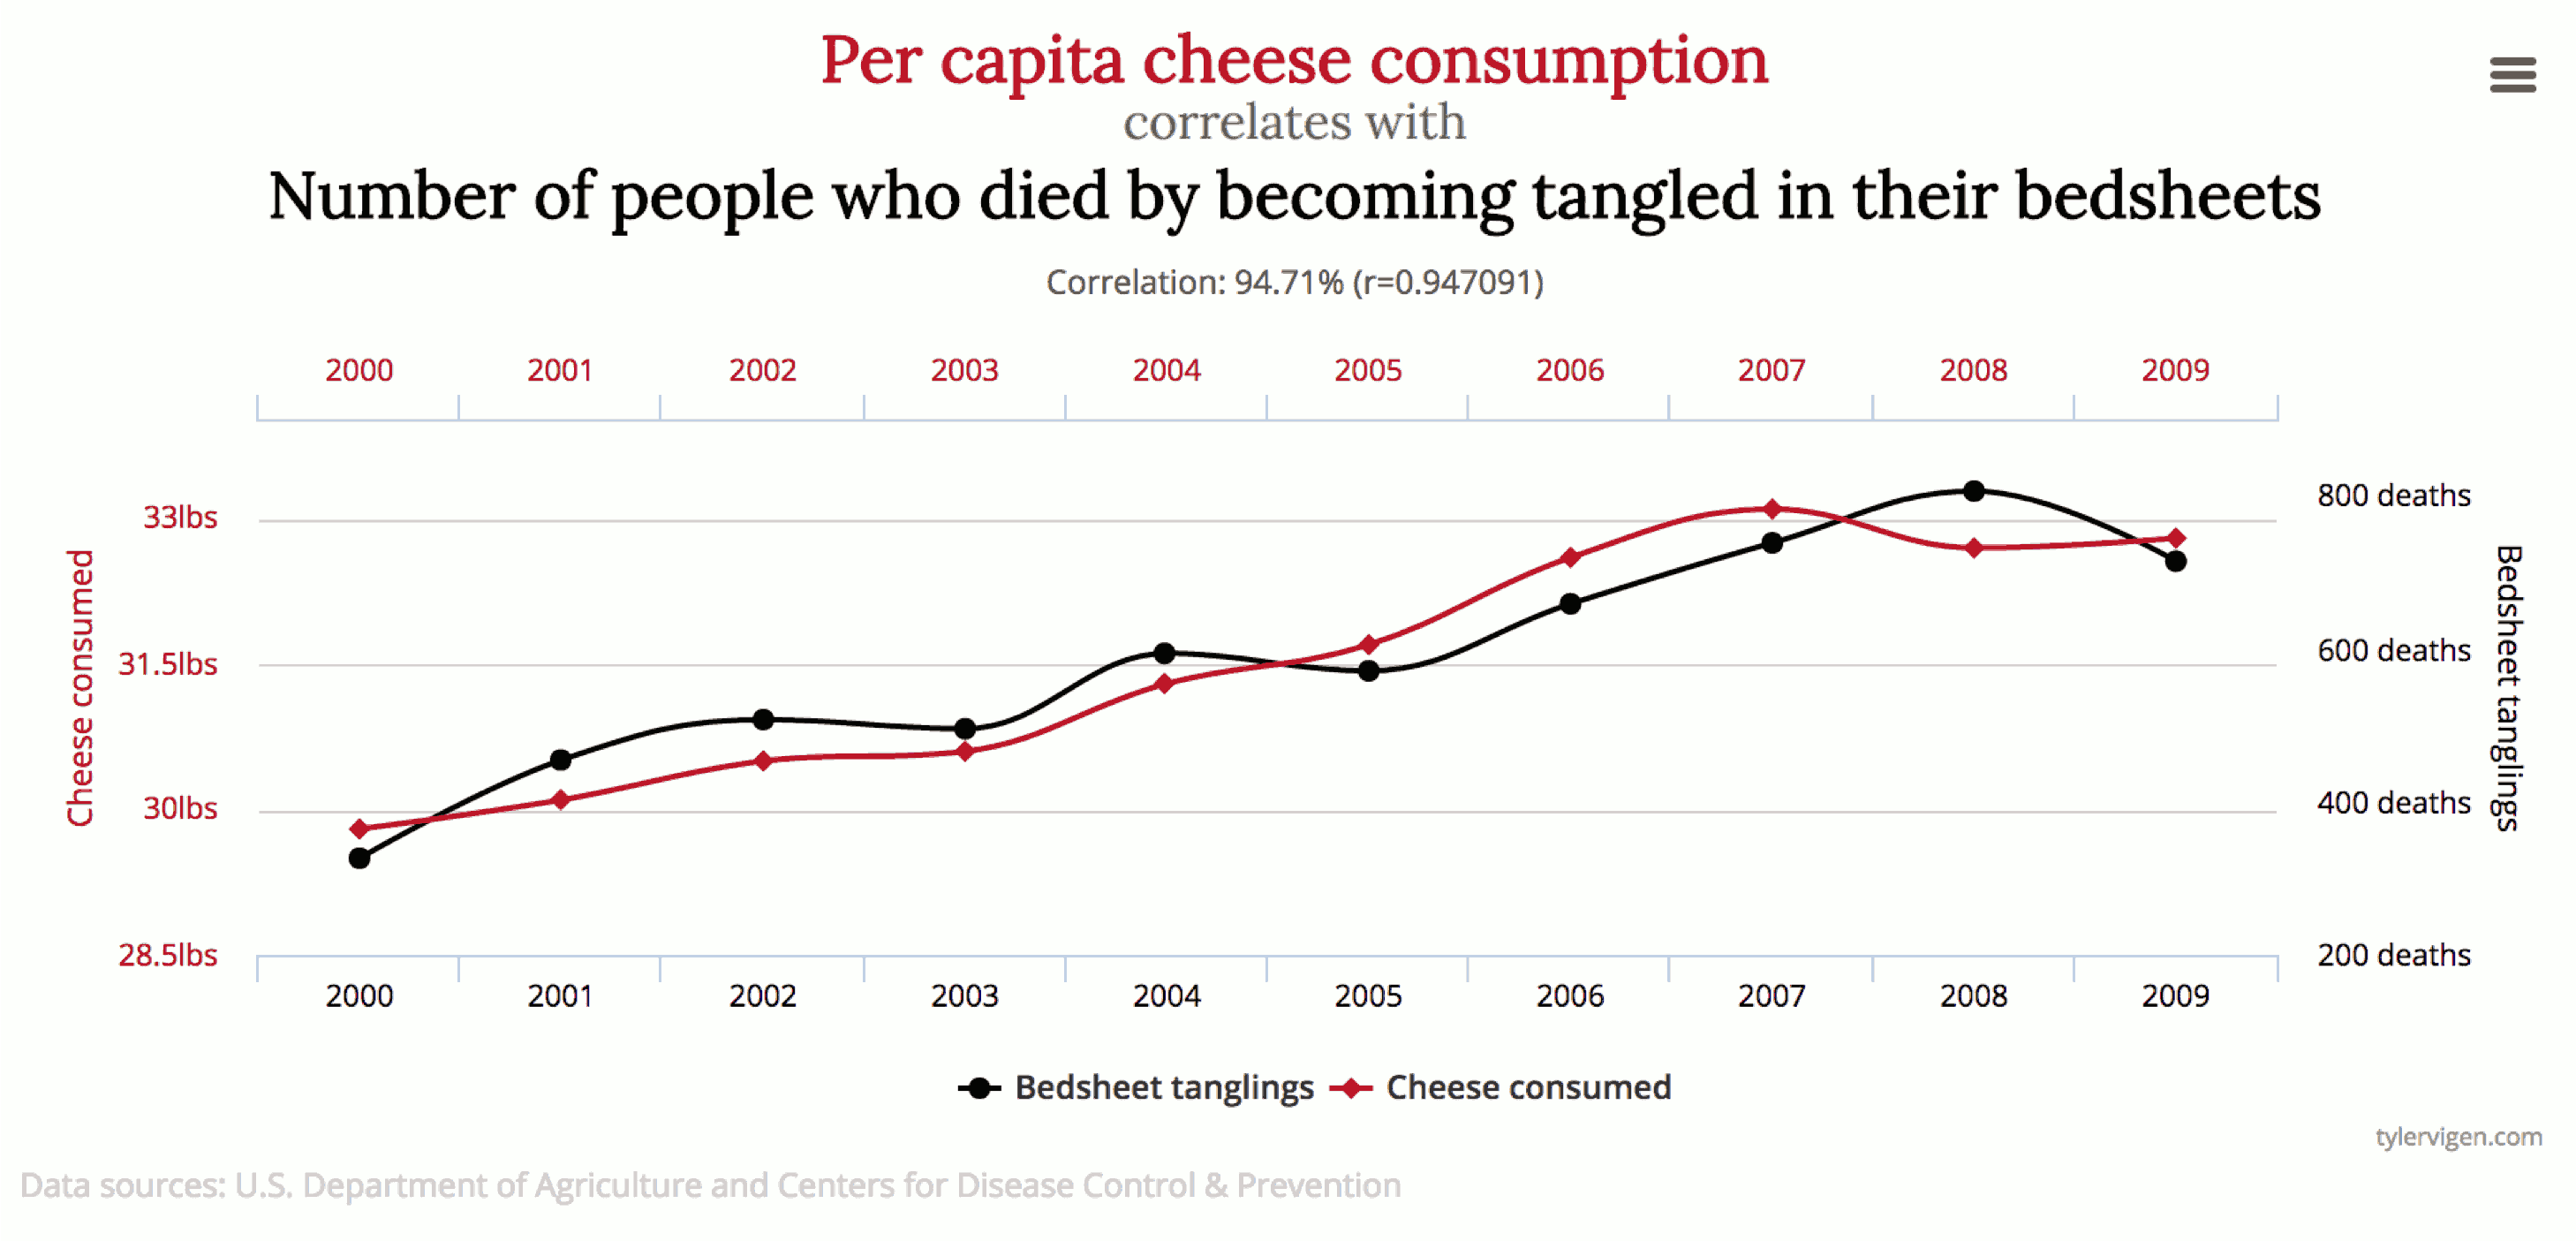
\includegraphics[width=0.99\textwidth]{fig/cheese}
\end{frame}

\begin{frame}{Correlation vs causation}
Variables X and Y vary together

\begin{block}{Causality vs correlation:}
Does movement in X ``cause''
movement in Y in some metaphysical sense?
\end{block}

Hard to test with \emph{observation} alone;\\
\emph{experimental} interventions provide much stronger evidence.
\pause

\begin{itemize}
    \item Meaningful relationship: requires causal mechanism \\
        (\emph{why/how} does X cause Y?)
    \item Simultaneous variation ``induced'' \\
        by the variation of a common third effect
    \item Spurious (accidental) correlation
\end{itemize}
\end{frame}

\begin{frame}{Summary: two variables}
In general: Look at the data! 

\vspace{1em}
Two \structure{continuous} variables:
\begin{enumerate}
    \item Make a scatter plot
    \item Compute correlation
    \item Think carefully whether the relation is meaningful!
\end{enumerate}
\end{frame}


